
\subsection{2分ヒープ}
\frame{
  \frametitle{2分ヒープ}
  \begin{block}{Binary Heap}
    全順序集合$P(C,\leq)$について,$C$上の要素からなるヒープは\\
    以下の操作が実行できる
    \itemize{
    \item push : $O(\log N)$で$C$の要素$x$を追加する
    \item replace : $O(\log N)$で$C$の要素$x$でヒープの最大値をもつ要素を置き換える
    \item pop : $O(\log N)$でヒープの最大値をもつ要素を削除する
    \item delete : $O(\log N)$で与えられたポインタの先の要素を消去する
    \item top : $O(1)$でヒープの最大値を求める\\
    }
    ヒープ条件を満たす完全二分木の構造\\
    (二分木:出次数が高々2の有向木)\\
    (完全二分木:出次数が0か2で,全ての葉が同じ深さ)
  \end{block}
}

\frame{
  \frametitle{2分ヒープ}
  \begin{alertblock}{ヒープ条件}
    \center{
      全ての要素の値はその親の要素の値より小さいか等しい
    }
  \end{alertblock}
  \begin{exampleblock}{例}
    \center{
      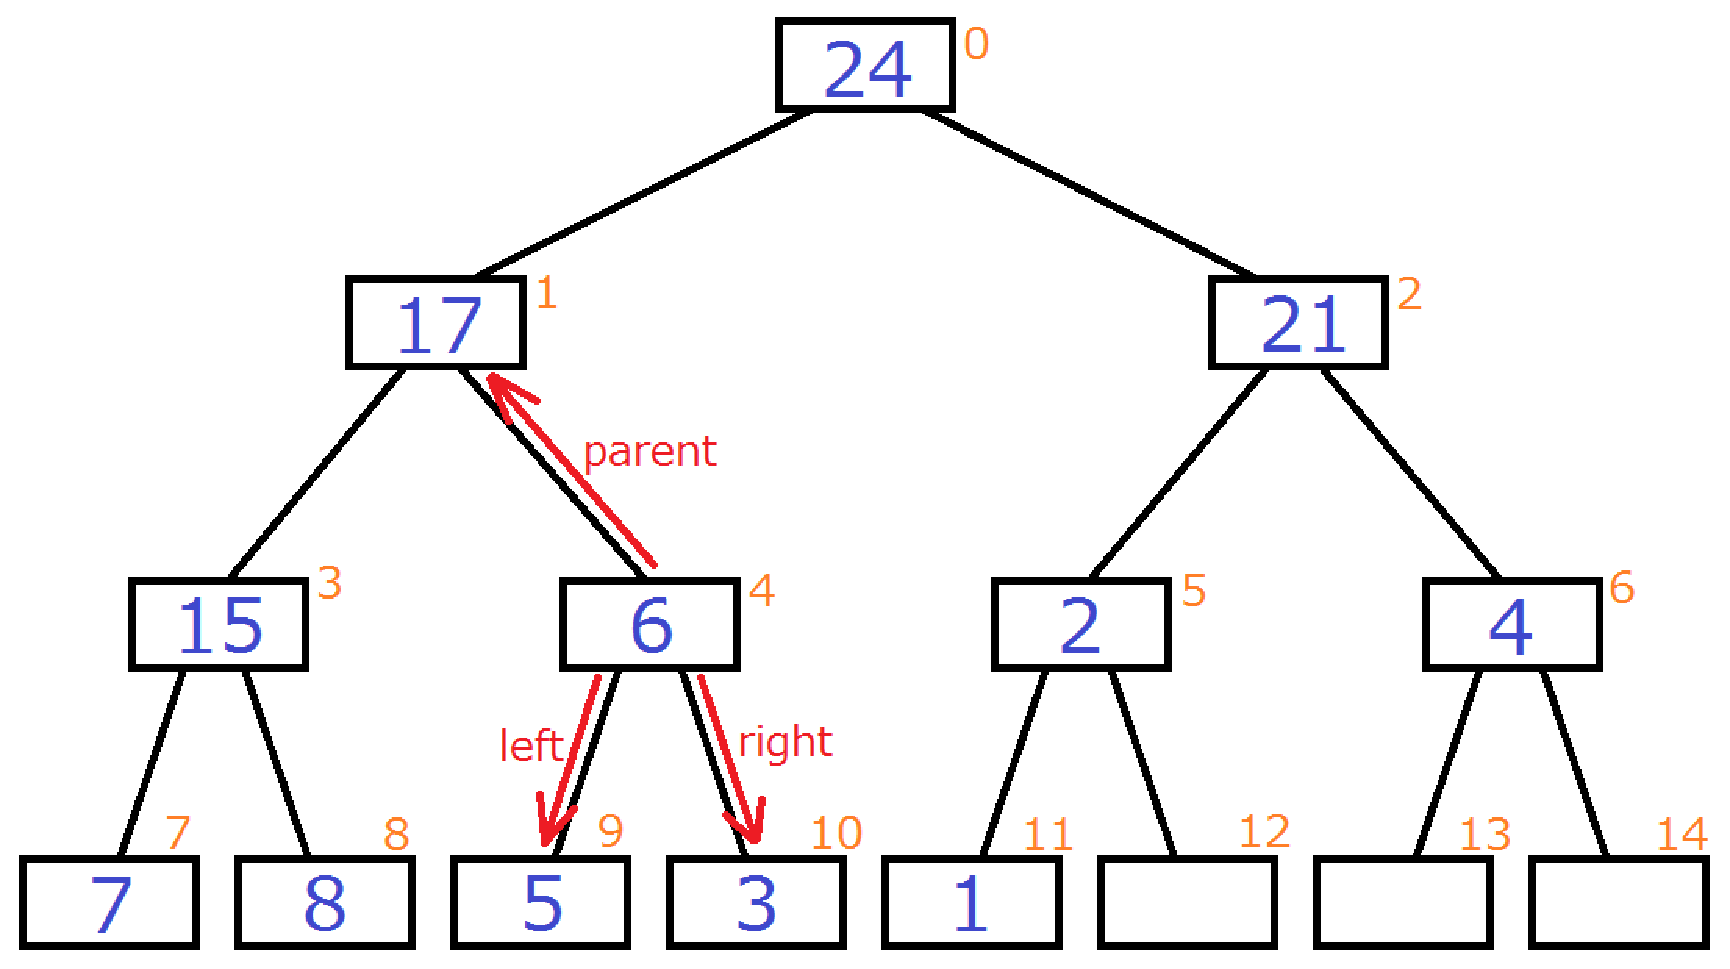
\includegraphics[width=8cm]{image/heap01.pdf}
    }
  \end{exampleblock}
}

\frame{
  \frametitle{key, parent, left, right}
  2分ヒープAについて
  \begin{block}{key($i$)}
    1.  {\bf If} $i < size(A)$\\
    2. ~~ {\bf Then} return $key[i]$\\
    3. ~~ {\bf Else} return $-\infty$
  \end{block}
  \begin{block}{parent($i$)}
    1.  return $(i-1)/2$
  \end{block}
  \begin{block}{left($i$)}
    1.  return $2i+1$
  \end{block}
  \begin{block}{right($i$)}
    1.  return $2i+2$
  \end{block}
}

\frame{
  \frametitle{push}
  \begin{block}{push$(A, k)$}
    1.  $i \leftarrow size[A]$\\
    2.  $size[A] \leftarrow size[A] + 1$\\
    3.  {\bf While} $i > 0$ かつ $key(parent(i)) < k$ {\bf do}\\
    4. ~~ $key[i] \leftarrow key(parent(i))$\\
    5. ~~ $i \leftarrow parent(i)$\\
    6.  $key[i] \leftarrow k$
  \end{block}
}

\frame{
  \frametitle{push}
  \begin{block}{push}
    \center{
      $O(\log N)$で$C$の要素$x$を追加する
    }
  \end{block}
  \begin{exampleblock}{例}
    \center{
      \includegraphics<1>[width=8cm]{image/heap02.pdf}
      \includegraphics<2>[width=8cm]{image/heap03.pdf}
      \includegraphics<3>[width=8cm]{image/heap04.pdf}
    }
  \end{exampleblock}
}

\frame{
  \frametitle{replace}
  \begin{block}{replace$(A, k)$}
    1.  $key[0] \leftarrow k$\\
    2.  $i \leftarrow 0$\\
    3.  {\bf While} $key(i) < key(left(i))$ or $key(i) < key(right(i))$ {\bf do}\\
    4. ~~ {\bf If} $key(left(i)) > key(right(i))$\\
    5. ~~~~~ {\bf Then} $child \leftarrow left(i)$\\
    6. ~~~~~ {\bf Else} $child \leftarrow right(i)$\\
    7. ~~ $key[i] \leftrightarrow key[child]$\\
    8. ~~ $i \leftarrow child$
  \end{block}
}

\frame{
  \frametitle{replace}
  \begin{block}{replace}
    \center{
      $O(\log N)$で$C$の要素$x$ヒープの最大値をもつ要素を置き換える
    }
  \end{block}
  \begin{exampleblock}{例}
    \center{
      \includegraphics<1>[width=8cm]{image/heap05.pdf}
      \includegraphics<2>[width=8cm]{image/heap06.pdf}
      \includegraphics<3>[width=8cm]{image/heap07.pdf}
    }
  \end{exampleblock}
}

\frame{
  \frametitle{pop}
  \begin{block}{pop$(A, k)$}
    1.  $x \leftarrow key(size[A]-1)$\\
    2.  $size[A] \leftarrow size[A]-1$\\
    3.  replace$(A, x)$
  \end{block}
}

\frame{
  \frametitle{pop}
  \begin{block}{pop}
    \center{
      $O(\log N)$でヒープの最大値をもつ要素を削除する
    }
  \end{block}
  \begin{exampleblock}{例}
    \center{
      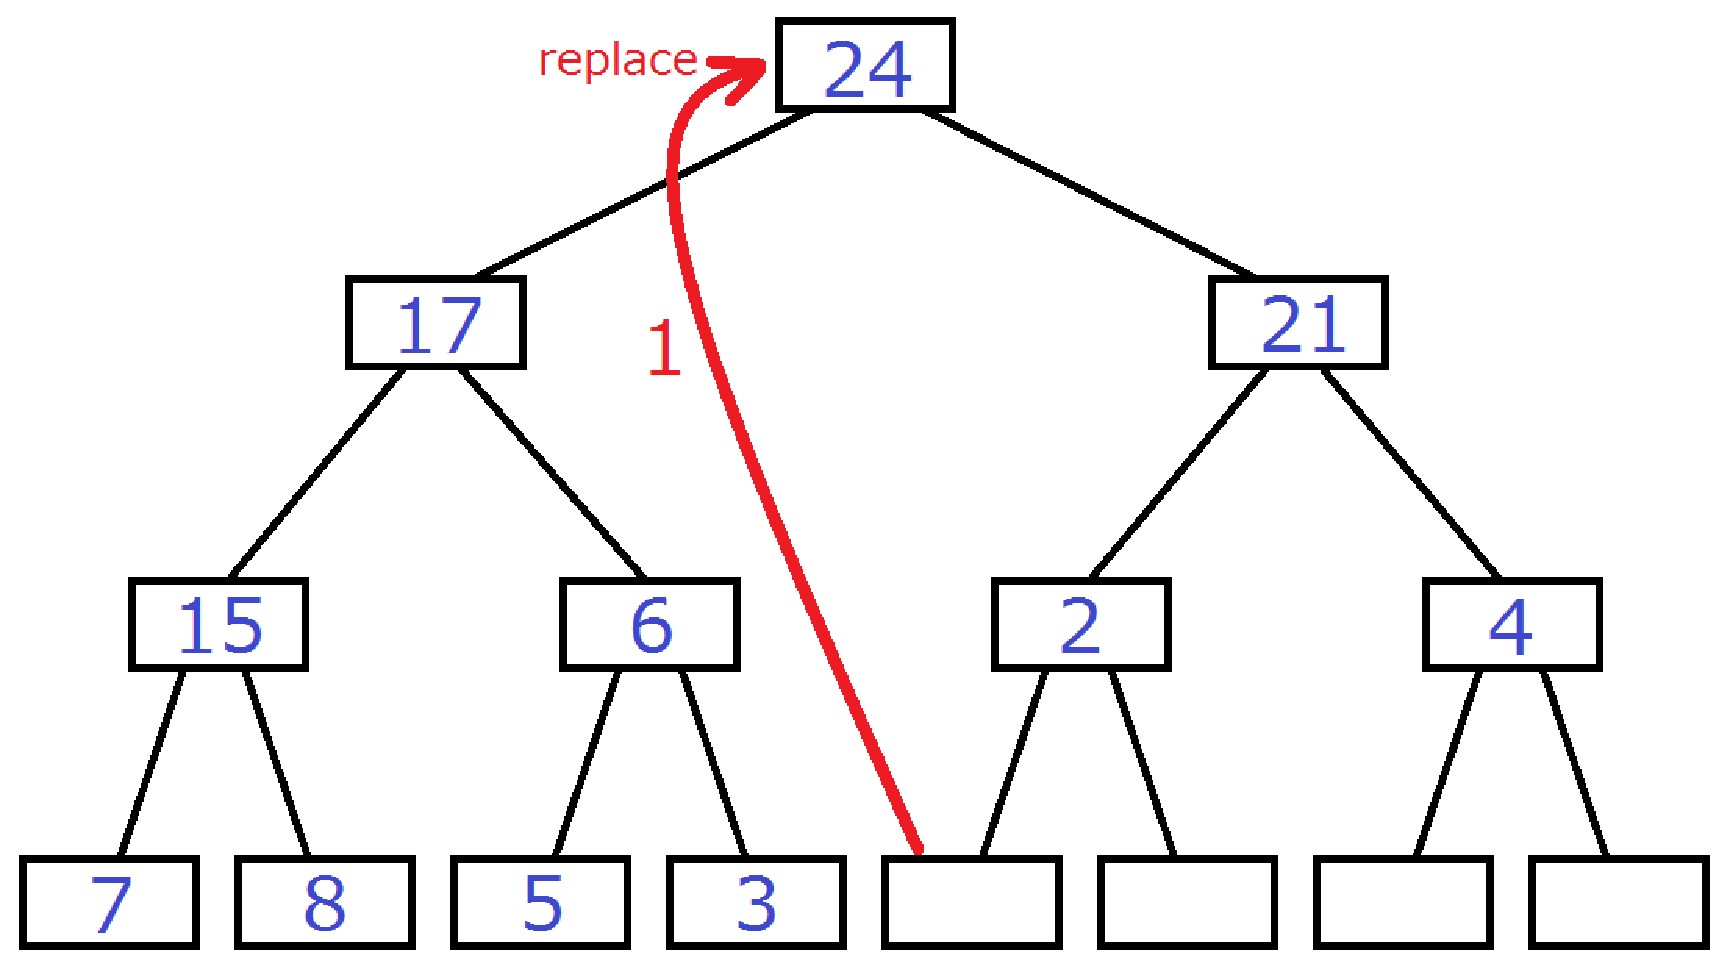
\includegraphics[width=8cm]{image/heap08.pdf}
    }
  \end{exampleblock}
}

\frame{
  \frametitle{delete}
  \begin{block}{delete}
    \center{
      $O(\log N)$で与えられたポインタの先の要素を消去する
    }
  \end{block}
  \begin{exampleblock}{例}
    \center{
      \includegraphics<1>[width=8cm]{image/heap09.pdf}
      \includegraphics<2>[width=8cm]{image/heap10.pdf}
      \includegraphics<3>[width=8cm]{image/heap11.pdf}
      \includegraphics<4>[width=8cm]{image/heap12.pdf}
      \includegraphics<5>[width=8cm]{image/heap13.pdf}
    }
  \end{exampleblock}
}

\frame{
  \frametitle{top}
  \begin{block}{top$(A)$}
    1.  {\bf If} $size(A) > 0$\\
    2. ~~ {\bf Then} return $key(0)$\\
    3. ~~ {\bf Else} return $undefined$
  \end{block}
}

\frame{
  \begin{block}{Binary Heap}
    \itemize{
    \item push : $O(\log N)$で$C$の要素$x$を追加する
    \item replace : $O(\log N)$で$C$の要素$x$でヒープの最大値をもつ要素を置き換える
    \item pop : $O(\log N)$でヒープの最大値をもつ要素を削除する
    \item delete : $O(\log N)$で与えられたポインタの先の要素を消去する
    \item top : $O(1)$でヒープの最大値を求める\\
    }
  \end{block}
  \begin{alertblock}{ヒープは便利!!}
    ヒープを始めとする高速な優先度付きキューはあらゆる場面で活躍する
  \end{alertblock}
  \only<2>{しかしこれだけでは終わらない} \\
}
